%%%%                %%%%
%%%% BASES TEÓRICAS %%%%
%%%%                %%%%

\chapter{Bases teóricas}
\label{chap:bases-teoricas}

\lettrine{E}l objetivo de este capítulo es sentar las bases tecnológicas y teóricas sobre las que se ha llevado a cabo el proyecto. En particular, se expone de qué manera se consiguen las coordenadas de las palabras y qué tecnologías intervienen para la obtención de la salida en formato estructurado.

Las aplicaciones comerciales utilizan las ubicaciones para seleccionar contenidos relevantes. Lo habitual es que el usuario pueda marque rectángulos sobre las páginas y los procesos de extracción y verificación únicamente tengan en cuenta estas áreas. Para poder hacer esto se necesitan las localizaciones de las palabras, pares clave-valor, tablas, etc. Entre los PDF manejados para la elaboración de este trabajo hay dos categorías importantes: aquellos que tienen texto directamente extraíble y otros donde cada página es una imagen. El primer caso es el habitual en los PDF generados con procesadores de textos u otros software. Se puede comprobar fácilmente si un PDF contiene texto directamente extraíble abriendo el documento con un visor y realizando la selección con el ratón. Si es el caso, se puede evitar hacer OCR del documento y obtener una versión sin errores del texto.

\section{Software para la manipulación de PDF}

Existen librerías y también aplicaciones capaces de manipular ficheros PDF para extraer texto, imágenes, reordenar páginas y otras muchas posibilidades. Para los objetivos del proyecto, sería necesaria una herramienta capaz de extraer el texto pero también sus coordenadas sobre el documento. Se revisaron varias alternativas, como PDFBox 
\footnote{https://pdfbox.apache.org/}, Win2PDF 
\footnote{https://www.win2pdf.com/doc/command-line-extract-text-pdf.html}, ebook-convert 
\footnote{https://manual.calibre-ebook.com/es/generated/es/ebook-convert.html}, que forma parte de la aplicación Calibre, y pdftotext 
\footnote{https://poppler.freedesktop.org/}. Únicamente esta última ofrece la posibilidad de generar las localizaciones necesarias.

La implementación original de esta utilidad fue realizada por Glyph \& Cog, autores del visor Xpdf. En el año 2005 surge la librería Poppler a partir del fork de la versión 3.0.3 de Xpdf. Esta es la implementación disponible mayormente en las distribuciones Linux. Por ejemplo, en Ubuntu se puede instalar con el paquete \verb|poppler-utils| e incluye otras muchas herramientas relacionadas.

Cuando se invoca la herramienta con el parámetro \verb|-bbox| se genera una salida en lenguaje XHTML. Esta variante del HTML tiene la ventaja de ser admitida por cualquier parser XML. Se identifican tags para los elementos que representan bloques, lineas y palabras. En cada uno se informa con cuatro valores de la localización del rectángulo que engloba al elemento: \emph{xMin}, \emph{xMax}, \emph{yMin}, \emph{yMax}. La generación de información de coordenadas o bounding box, además del texto, existe gracias a una aportación al proyecto del año 2010 de Kenneth Berland. 

\begin{figure}[hp!]
    \centering
    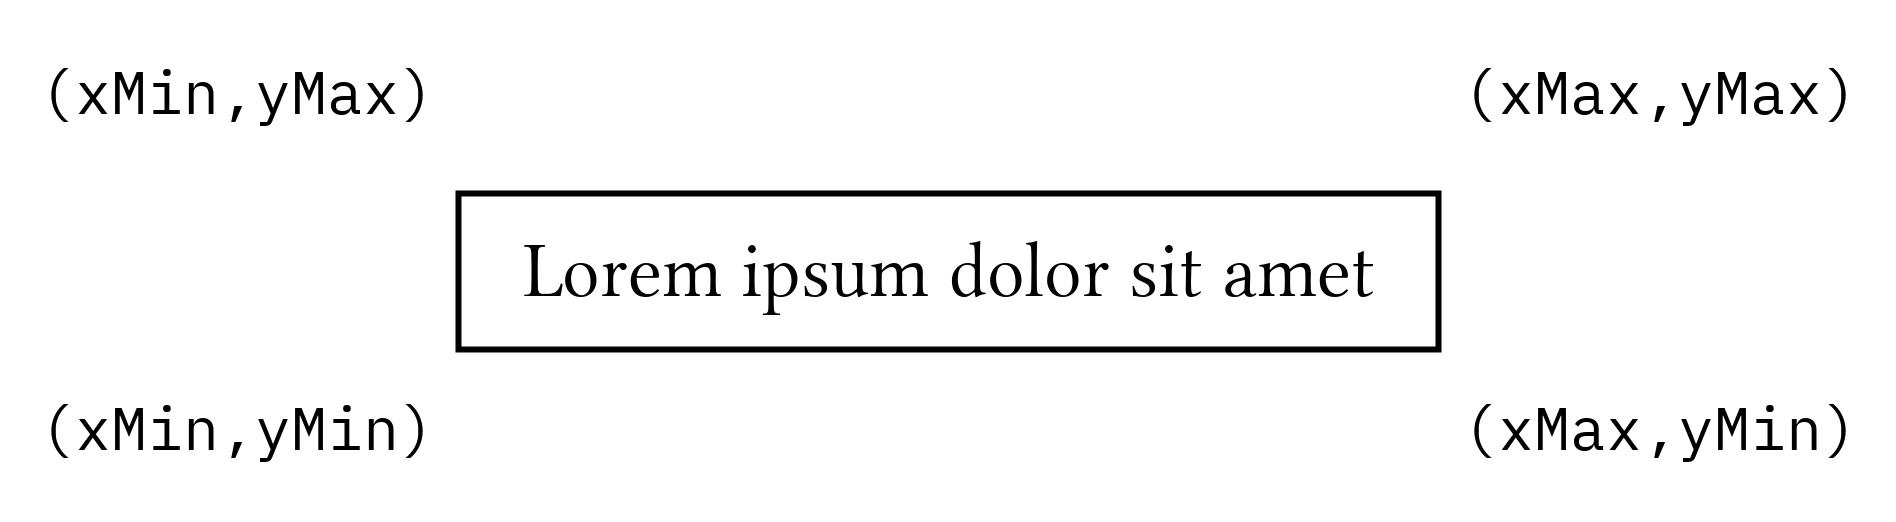
\includegraphics[width=0.75\textwidth]{imaxes/c-bases-teoricas/correspondencia-coordenadas-bounding.png}
    \caption{Correspondencia de las coordenadas en una bounding box}
    \label{fig:bounding-box}
\end{figure}

Una limitación común en todas estas utilidades consiste en no respetar el layout del texto, tal como aparece en el documento original. Esto implica que algunos elementos pueden aparecer antes que otros en la información extraída. Otro problema es que hay palabras que aparecen con caracteres intermedios, espacios, por ejemplo, que no se ven en el PDF. Estas limitaciones se derivan del propio funcionamiento del formato PDF.

\section{El formato PDF}

PDF es un formato digital para la creación de documentos. Fue introducido por Adobe Systems en 1993. En los siguientes años, el uso de este formato se extendió por toda la sociedad, tanto en el ámbito público como en el privado. En el año 2008, la ISO publicó el estándar 32000-1, tomando como base especificación de PDF en su versión 1.7, creada y liberada por Adobe. Posteriormente se publicó la versión 2.0 como ISO 32000-2 en el año 2017 y más recientemente una actualización en el año 2020. PDF es un modelo de representación de imágenes que deriva del lenguaje PostScript, también desarrollado por Adobe. En PDF, el modelo de imagen admite gráficos y texto de forma independiente al dispositivo de salida.

% TODO Considerar si añadir más información de PostScript.

\subsection{Almacenamiento de información}

Un PDF no es un fichero de texto, es un fichero binario de 8 bits con una estructura interna determinada. Sus elementos básicos son los objetos. Cualquier información que se visualice en el documento existirá realmente como un objeto dentro del fichero. Estos objetos están serializados dentro del fichero y pueden ser de alguno de los siguientes nueve tipos:

\begin{enumerate}
    \item \textbf{Null}: se utiliza para indicar la ausencia de un valor.
    \item \textbf{Boolean}: indica los valores de verdad true o false.
    \item \textbf{Integer}: representa valores enteros. Puede aparecer como \verb|1|, \verb|+2|, \verb|-100|.
    \item \textbf{Real}: representa valores decimales y puede aparecer como \verb|0,05|, \verb|.25|, \verb|-3,1415|.
    \item \textbf{Name}: son secuencias únicas dentro del fichero, comienzan con una barra. Por ejemplo: \verb|/Type|, \verb|/ThisIsName|.
    \item \textbf{String}: puede ser de 4 tipos:
    \begin{itemize}
        \item ASCII: bytes codificados en ASCII.
        \item PDFDocEncoded: bytes codificados con la codificación PDFDocEncoding.
        \item Text: bytes codificados en PDFDocEncoding o UTF-16BE.
        \item Date: utilizado para fechas. Se codifican en ASCII con un patrón de fecha. \footnote{D:YYYYMMDDHHmmSSOHH’mm}.
    \end{itemize}
    \item \textbf{Array}: es una colección heterogénea de objetos. Se escriben entre corchetes: \verb|[ 0 20 (E) ]|.
    \item \textbf{Dictionary}: es una tabla asociativa que contiene pares clave/valor. Pueden contener valores anidados y es utilizado para crear la jerarquía de todos los objetos del documento. Para indicar el comienzo y fin se utilizan los símbolos \verb|<<| y \verb|>>|. Las claves se indican con valores de tipo name.
    \item \textbf{Streams}: son secuencias de bytes de 8 bits sin límite de tamaño. Son utilizados para almacenar cualquier información binaria, por ejemplo imágenes, ficheros JSON o tipografías. Los stream tienen como preámbulo un diccionario de propiedades del stream. Este diccionario siempre debe contener, al menos, la clave \verb|/Length| que indica en bytes el tamaño del stream. Otra clave importante es \verb|/Filter|. \verb|/Filter| indica que la información está comprimida o codificada. Las imágenes se suelen codificar como DCTDecode o JPXDe que son versiones diferentes del formato JPEG. Para otro tipo de datos está disponible el algoritmo FlateDecode, similar a  DEFLATE, el mismo utilizado en los ficheros ZIP.
\end{enumerate}

Los objetos presentados hasta el momento son los objetos directos. Los objetos directos tienen el valor almacenado en el propio objeto. También existen los objetos indirectos que se referencian indirectamente y el consumidor tiene que saltar a otra posición en el fichero. Los objetos indirectos tienen un identificador único dentro del fichero. Las referencias son de la forma: \verb|/ObjIndirecto  5 0 R|.

\subsection{Estructura en un fichero}

La estructura de un fichero está dividida en cuatro partes, tal como se muestra en la figura \ref{fig:secciones-pdf}: header, body, cross-reference table y trailer. El header tiene al menos dos líneas. La primera se utiliza para indicar que el fichero es un PDF y la versión del estándar que le corresponde. La segunda es simplemente un separador: \verb|%%EOF|. 

\begin{figure}[hp!]
    \centering
    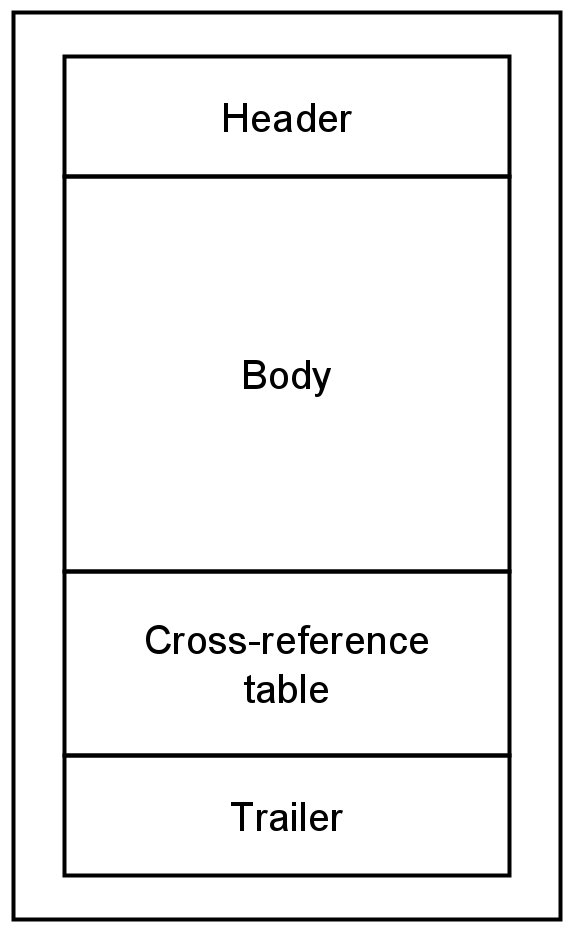
\includegraphics[width=0.3\textwidth]{imaxes/c-bases-teoricas/secciones-de-un-pdf.png}
    \caption{Las cuatro secciones de un PDF}
    \label{fig:secciones-pdf}
\end{figure}

El trailer es un objeto de tipo diccionario. Contiene claves y valores que aportan información a nivel de documento. Hay dos claves especialmente importantes, /Size que indica el número de entradas de la Cross-reference table y /Root que apunta al objeto que contiene el comienzo del Catálogo. El body contiene el objeto del Catálogo y todos los demás objetos que conforman el contenido del fichero PDF. La Cross-Reference Table es un índice de todos los objetos indirectos del PDF. Se utiliza para implementar la navegación sobre el fichero. Contiene la información necesaria para poder realizar saltos a la posición donde se encuentra el objeto que se quiere leer. La versión tradicional tiene tres columnas y la secuencia de entradas hace referencia al número del objeto buscado. En el ejemplo, para encontrar el objeto 2, tercera entrada, hay que saltar hasta el byte 32800:

%\begin{minted}
0000000000 65535 f\\
0000000009 00000 n\\
0000032800 00000 n\\
0000000203 00000 n\\
0000000298 00000 n\\
0000008654 00000 n\\
0000000335 00000 n
%\end{minted}

% TODO Considerar hablar del catálogo o dejarlo para la parte de implementación.

%%%%%

\section{Representación de coordenadas en orígenes OCR}

La representación de las localizaciones de los elementos identificados por el proceso OCR es solo una parte de toda la información que se genera como salida de un engine. Existen varias propuestas de formatos que se proponen como formatos abiertos con intención de favorecer su adopción. Es el caso de hOCR \cite{ocrRepres_hocr_breuel_spec}, ALTO \cite{ocrRepres_alto_spec}, PAGE \cite{ocrRepres_page_pletschacher_paper} y TEI \cite{ocrRepres_tei_project}. Los tres últimos emplean XML como base y definen las etiquetas necesarias. La transformación entre ellos es posible y existe al menos un proyecto capaz de hacerlo
\cite{ocrRepres_conversion_ocrFileformat}. hOCR es el formato de representación escogido para el proyecto, como se verá en \ref{sec:rec-optico-caracteres}.

\subsection{El microformato hOCR}

hOCR es un estándar abierto que utiliza HTML como base tecnológica. Se diseñó siguiendo el modelos de los microformatos. Los microformatos son una tecnología ligada al auge de los blogs durante el año 2004. Su objetivo es aportar significado semántico a construcciones HTML, que de otro modo no lo tendrían ya que no forman parte como tal del lenguaje. La especificación hOCR hace uso de etiquetas \verb|DIV| y \verb|SPAN| para los elementos. Para la información se utilizan atributos como \verb|class|, \verb|title| o \verb|style|. Se combina con CSS para ampliar las capacidades del HTML en cuanto a representación de la salida OCR. HTML tiene soporte nativo para muchas características habituales en los documentos como estilo, tipografías, espaciado, etc.

La especificación hOCR define tres tipos de marcado:

\begin{itemize}
    \item Un marcado a \textbf{nivel lógico} que permite definir las secciones de un documento como en una estructura de tipo árbol.
    \item Un segundo tipo de marcado para representar el \textbf{nivel tipográfico y de división entre páginas}. Tiene la capacidad de modelar el documento de forma  que sus elementos principales se trasladarían al formato impreso de forma correcta. Este modelo se apoya en los procesos habituales que consideran el documento como un conjunto de bloques y elementos que se deben trasladar a su posición correcta.
    \item Un ultimo tipo para el \textbf{nivel físico} representado por líneas, figuras, y las palabras. Es específico para la implementación de cada motor de OCR. 
\end{itemize}

El formato proporciona también información geométrica, posiciones, de las palabras y valores de confianza respecto a la calidad que el motor valora sobre el reconocimiento realizado.

\section{Reconocimiento Óptico de Caracteres}
\label{sec:rec-optico-caracteres}

Para realizar el Reconocimiento Óptico de Caracteres se seleccionó Tesseract \cite{ocr_tesseract_raysmithetal.TesseractocrTesseract2021}. Existen otros de fuente abierta que se pueden considerar:

\begin{itemize}
    \item \textbf{OCRopus} \cite{ocr_ocropus_ocropy_project}, \textbf{Kraken}  y \textbf{Calamary} \cite{ocr_calamari_journal}: OCRopus es una colección de herramientas más que un producto final. Kraken y Calamary son forks de OCRopus que proporcionan un producto final. Sin embargo los tres proyectos están enfocados en resolver el problema de reconocer textos históricos con tipografías clásicas. Revisando la documentación de los tres no se encontró modelos preentrenados en castellano.
    \item \textbf{EasyOCR} (\cite{ocr_easyocr_official}, \cite{ocr_easyocr_project}) es la alternativa más viable. Es un proyecto que se actualiza regularmente y tiene soporte comercial. Como punto negativo destaca que aunque proporciona información de bounding-box, no sigue ninguno de los estándares comentados con anterioridad.
\end{itemize}

\textbf{Tesseract} \cite{ocr_tesseract_smith_paper} es un engine de código abierto y desarrollado inicialmente por Hewlett Packard \cite{ocr_tesseract_v4_release_notes} entre los años 1985 y 1995. Después de un periodo sin actividad, en el 2006 el proyecto fue recuperado por Google, que lo mantiene desde entonces. Hoy en día tiene soporte para más de cien idiomas y la red neuronal que emplea \footnote{Desde la versión 4, Tesseract utiliza una red LSTM. Esta es una red neuronal de tipo recurrente o RNN} puede ser entrenada para casos específicos, si se necesita. Existe una amplia documentación en la web oficial, además, numerosos tutoriales en la red permiten familiarizarse con la herramienta. Es un proyecto bien conocido y de larga trayectoria.

\section{Detección de líneas tablas}

% TODO valorar si llevar esta sección a la implementación

La Transformada de Hough es una técnica de visión por computador utilizada para detectar figuras parametrizables, tales como líneas o círculos. El algoritmo parte de una imagen binaria que representa los bordes encontrados por una detector de bordes. A continuación se calculan todas las posibles líneas que podrían pasar por cada punto y se lleva a cabo una votación. Se seleccionan las líneas más votadas, entre todas las detectadas.

Este algoritmo proporciona una manera automática de localizar los bordes entre líneas de las tablas de muchos documentos y evita la necesidad de incorporar dicha información a las plantillas de forma manual. Se utiliza la implementación incluida en la librería OpenCV.

\section{Análisis léxico y sintáctico}

Flex y Bison son dos herramientas utilizadas en conjunto para construir analizadores sintácticos. ¿Qué es un analizador sintáctico?

La primera se utiliza para crear escáneres y la segunda para generar parsers. Ambas utilizan como entrada unos ficheros que definen las reglas válidas.
